\documentclass[../../../../main.tex]{subfiles}
\begin{document}

\begin{flushright}
\footnotesize\textit{【自動文字起こし・要確認】}
\end{flushright}

\begin{proof}[解]
(1) $f_1'(x) = 3x^2 - 3$ から下表をうる.

\begin{center}
\begin{tabular}{|c|ccccc|}
\hline
$x$ & $\dots$ & $-1$ & $\dots$ & $1$ & $\dots$ \\ \hline
$f_1'$ & $+$ & $0$ & $-$ & $0$ & $+$ \\ \hline
$f_1$ & $\nearrow$ & $2$ & $\searrow$ & $-2$ & $\nearrow$ \\ \hline
\end{tabular}
\end{center}

よってグラフは右上図. したがって,
\[
\begin{cases}
|a| > 2 \text{ の時 } 1 \text{ 個} \\
|a| = 2 \text{ の時 } 2 \text{ 個} \\
|a| < 2 \text{ の時 } 3 \text{ 個}
\end{cases} \quad \text{//}
\]

\medskip
(2) (1)と同様にして,
\[
\begin{cases}
|a| > 2 \text{ の時 } 1 \text{ 個} \\
|a| = 2 \text{ の時 } 5 \text{ 個} \\
|a| < 2 \text{ の時 } 9 \text{ 個}
\end{cases} \quad \text{//}
\]

\medskip
(3) $f_n(x) = a \ (|a| < 2)$ を満たす実数 $x$ が $3^n$ 個である $\dots \diamondsuit$ ことを帰納的に示す.

$n=1$ の時は(1)から成立するので, 以下 $n=k \in \mathbb{N}$ での成立を仮定する. $f_{k+1}(x) = a$ なる $f_k(x)$ は (1)のグラフより $-2 < f_k(x) < 2$ に 3 つあるから, 仮定より $f_{k+1}(x) = a$ を満たす $x$ は $3^{k+1}$ 個ある.

よって $n = k+1$ でも $\diamondsuit$ は成立. したがって $\diamondsuit$ は示されたから, $a=0$ として題意の主張は示される. \qed
\end{proof}

\begin{center}
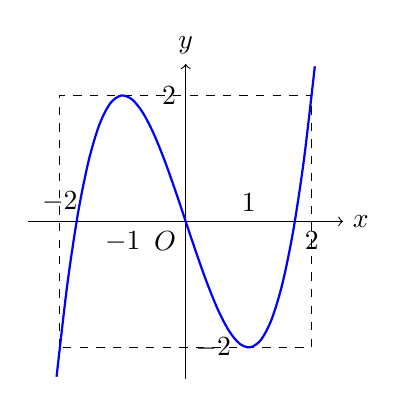
\begin{tikzpicture}[scale=0.8]
  \draw[->] (-2.5,0) -- (2.5,0) node[right] {$x$};
  \draw[->] (0,-2.5) -- (0,2.5) node[above] {$y$};
  \draw[dashed] (-2,-2) rectangle (2,2);
  \draw[domain=-2.05:2.05,smooth,variable=\x,blue,thick] plot ({\x},{\x*\x*\x - 3*\x});
  \node at (-1,0) [below] {$-1$};
  \node at (1,0) [above] {$1$};
  \node at (2,0) [below] {$2$};
  \node at (-2,0) [above] {$-2$};
  \node at (0,2) [left] {$2$};
  \node at (0,-2) [right] {$-2$};
  \node at (0,0) [below left] {$O$};
\end{tikzpicture}
\end{center}

\end{document}
